\chapter{Simulations (10 pgs)}

This part of thesis serves as a widen documentation for the \texttt{PyVort} codebase, a new approach to simulate quantum vortices. The code is written in well commented Python 3, arranged in a modular structure. The primary aim of this documentation is to highlight which module(s) are involved and how they work.
In appendix, one can find a table of the parameters which can be set in the \texttt{main.py} file.

To run the code, there has to be only installed Python 3 (with dependencies) on any OS. All the Python code can be found in the directory \texttt{src/}. The entire project is open-source and can be found as a public GitHub repository. Pull requests of any further development would be definitely appreciated.

\section{Vortex filament model}
\begin{itemize}
	\item FD order, radius
	\item Vandermonde vs analytical method
	\item comp complexities of LIA and Biot-Savart
	\item coords and velocities updating
\end{itemize}

The \texttt{PyVort} code is based on vortex filament (VF) model, a technique pioneerd by Schwarz in the early 1980s. Superfluid vortex filament is represented by a series of mesh points distributed along the centerline of the VF. The motion of the whole VF is summed up by the motion of each mesh point.

\todo vortex picture

More precisely we define the VF as a three dimensional curve
$\vec{s}(\xi, t)$. Here $\xi$ represents arc-lengths and $t$ is time. Each mesh point is given by its coordinates $\vec{s}$, direct neighbour indices (previous and next mesh point). This resolves in a directed digraph, which a good starting point for the initial data structure.

We can construct the tangent vector $\vec{s}^{\prime}$, then normal vector, $\vec{s}^{\prime\prime}$, and the binormal vector, $\vec{s}^{\prime} \times \vec{s}^{\prime\prime}$ by taking numerical derivatives. Note $\vec{s}^{\prime} = \text{d}\vec{s} / \text{d}\xi$,
and so on. We denote the velocity at a point $\vec{s}$ as $\vec{v}(\vec{s})$ and consider the velocity field to be made up of two parts:

\begin{equation}
\vec{v} = \vec{v}_s + \vec{v}_n
\end{equation}

At present the code can be run only with infinite boundary conditions. Therefore, only closed-loop vortices can be realized using simulation.

\subsection*{State definition}

In Python 3, the implementation of VF is represented using \texttt{class} structure with following properties:

\begin{itemize}
	\item \underline{coordinates} - an array of coordinates arrays for each mesh point. In initialisation process, we can shape it arbitrarily.
	\item \underline{previous/next neighbour} - the array indices of one \textit{previous} and one \textit{next} mesh point according to the distance.
	\item \underline{LIA velocity} - calculation of self-induced velocity driven by the near surounding.
	\item \underline{BIOT velocity} -calculation of self-induced velocity driven by the farther parts of VF.
	\item \underline{Full velocity} - the sum of LIA velocity, BIOT velocity and the quantum parts (see the Schwarz's equation).
\end{itemize}

\todo code snipped of vortex class init

We will call this set of properties as a \textit{state} of VF.

\subsection{Finite differences}

Numerical derivatives $\vec{s}^{\prime\prime}$ and $\vec{s}^{\prime\prime\prime}$ need to be properly calculated. At a particular point on the VF, with position $\vec{s}_i$ , we define the distance to the particle in-front $\vec{s}_{i+1}$ as
$l_{+}$ and the distance to the particle behind $\vec{s}_{i-1}$ as $l_{-}$. By in-front/behind we refer to the particles next/previous
along the filament. Similarly, we can define the $l_{++}$ and $l_{--}$ for the farther particles, and so on.

Using finite differences theorem, we can construct the approximations for the first and second derivatives
$\vec{s}_i^{\prime}$, $\vec{s}_i^{\prime\prime}$ by taking the Taylor's series expansions. The resulting form is:

\begin{equation}
\frac{\text{d}^n\vec{s}_i}{\text{d}\xi^n} \approx
A\vec{s}_{i-2} + B\vec{s}_{i-1} + C\vec{s}_{i} + D\vec{s}_{i+1} + E\vec{s}_{i+2}
\hspace{1cm}
\text{for} \,n\in\{1,2\}
\end{equation}

\begin{figure}[h]
	\centering
	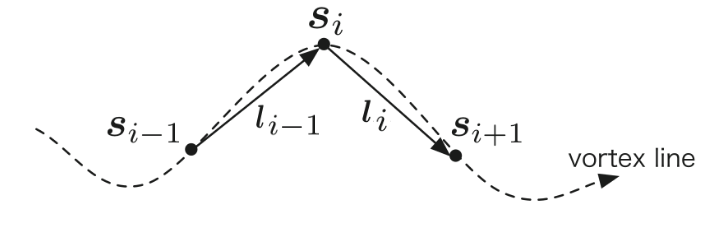
\includegraphics[width=0.8\textwidth]{graphics/simul/finite-diff}
	\caption{abcd}
\end{figure}







\section{Integration}
\begin{itemize}
	\item Euler vs. RK4 step
	\item time stepping
	\item stability
\end{itemize}

\section{Resegmentation}
\begin{itemize}
	\item adding and removing segments
	\item local spline
\end{itemize}

Points along the line are added (or removed) if the vortex is stretched (or compressed).

\section{Vortex ring}
\begin{itemize}
	\item initialisation
	\item movement, decreasing radius
	\item comparison with theory
	\item Kelvin waves (?)
\end{itemize}

\section{Future implementations}

If any two lines become very close (a distance less than the separation along the line) then the filaments reconnect, changing the topology of the system.

\newpage
